\documentclass[10pt,a4j,dvipdfmx]{jarticle}
%---------------------------------------------------
\usepackage{hyperref}
\usepackage{pxjahyper}
\usepackage{bm}
\usepackage{graphicx}
\usepackage{amssymb,amsmath}
\usepackage{ascmac}
\usepackage{float}
\usepackage{setspace}
\usepackage[dvips,usenames]{color}
\usepackage{colortbl}
\usepackage{algorithm}
\usepackage{algorithmic}
\usepackage{setspace}
\usepackage{subfigure}
\usepackage[deluxe,bold]{otf}
\usepackage[haranoaji]{pxchfon}
\usepackage{redeffont}
\usepackage{listings,jvlisting} %日本語のコメントアウトをする場合jvlisting(もしくはjlisting)が必要
\usepackage{booktabs}
%---------------------------------------------------
\definecolor{bl}{rgb}{0.94,0.97,1}
\definecolor{gr}{rgb}{0.5,0.5,0.5}
% \makeatletter
% \def\section{\newpage\@startsection {section}{1}{\z@}{2.3ex plus -1ex minus -.2ex}{2.3 ex plus .2ex}{\Large\bf}}
% \makeatother
%---------------------------------------------------
\setlength{\textwidth}{160truemm}
\setlength{\textheight}{240truemm}
\setlength{\topmargin}{-14.5truemm}
\setlength{\oddsidemargin}{-0.5truemm}
\setlength{\headheight}{0truemm}
\setlength{\parindent}{1zw}
\setlength{\abovedisplayskip}{-2pt} % 数式上部のマージン
\setlength{\belowdisplayskip}{-2pt} % 数式下部のマージン
%---------------------------------------------------
\setstretch{1.2}
%---------------------------------------------------
\renewcommand{\subfigtopskip}{5pt}	% 図の上の隙間。上図の副題と下図の間。
\renewcommand{\subfigbottomskip}{0pt} % 図の下の隙間。副題と本題の間。
\renewcommand{\subfigcapskip}{-6pt}	% 図と副題の間
\renewcommand{\subcapsize}{\scriptsize} % 副題の文字の大きさ
\newcommand{\mysection}[1]{\vspace{-20pt}\section{#1}}
\newcommand{\mysubsection}[1]{\vspace{-20pt}\subsection{#1}}
\newcommand{\mysubsubsection}[1]{\vspace{-10pt}\subsubsection{#1}}
\renewcommand{\lstlistingname}{ソースコード}
%---------------------------------------------------
% ヘッダーとフッターの設定
\usepackage{fancyhdr}
\rhead{\leftmark}
\chead{}
\lhead{\rightmark}
\cfoot{\thepage}

\rfoot{}
\begin{document}
%---------------------------------------------------
\setlength{\abovedisplayskip}{1.5pt} 
\setlength{\belowdisplayskip}{0pt}
%---------------------------------------------------
%ここからソースコードの表示に関する設定
\lstset{
  basicstyle={\ttfamily},
  identifierstyle={\small},
  commentstyle={\smallitshape},
  keywordstyle={\small\bfseries},
  ndkeywordstyle={\small},
  stringstyle={\small\ttfamily},
  frame={tb},
  breaklines=true,
  columns=[l]{fullflexible},
  numbers=left,
  xrightmargin=0zw,
  xleftmargin=3zw,
  numberstyle={\scriptsize},
  stepnumber=1,
  numbersep=1zw,
  lineskip=-0.5ex
}
%ここまでソースコードの表示に関する設定
%---------------------------------------------------


\pagenumbering{arabic}
\pagestyle{fancy}
\setlength{\headheight}{5truemm}

\mysection{LTspiceについて}
\subsection{初期設定}
\begin{enumerate}
  \setlength{\parskip}{0cm} % 段落間
  \setlength{\itemsep}{0cm} % 項目間
  \item インストール \\
  LTspiceをアナログデバイセズのホームページからダウンロードする。
  \item コントロールパネルの設定
  \begin{itemize}
    \setlength{\parskip}{0cm} % 段落間
    \setlength{\itemsep}{0cm} % 項目間
    \item LTspiceを起動
    \item 「Control Panel」(金槌マーク) → 「Operation」タブ → 「Automatically delete. raw files」のチェックボックスにチェックを入れてOKをクリックする。
    \item 「Control Panel」(金槌マーク) →「Netlist Option」 タブ → 「Style/Convention」 → 「Convert 'μ' to 'u'」 にチェックが入っているか確認する。
    \item OKをクリックする。
  \end{itemize}

  \begin{figure}[htb]
    \begin{center}
    \subfigure[金槌マーク]{	% 副題なし
    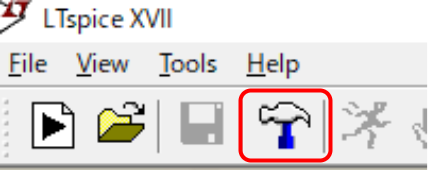
\includegraphics[width=.45\columnwidth]{img/1.png}
         }\\ % 改行
    \subfigure[Operationタブ]{
    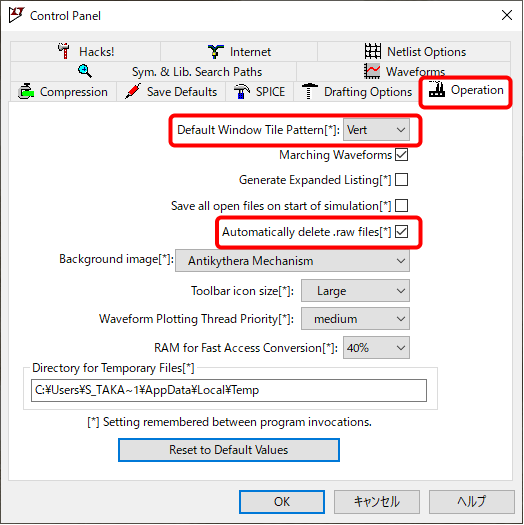
\includegraphics[width=.4\columnwidth]{img/2.png}
    }~
    \subfigure[Netlist Optionタブ]{
    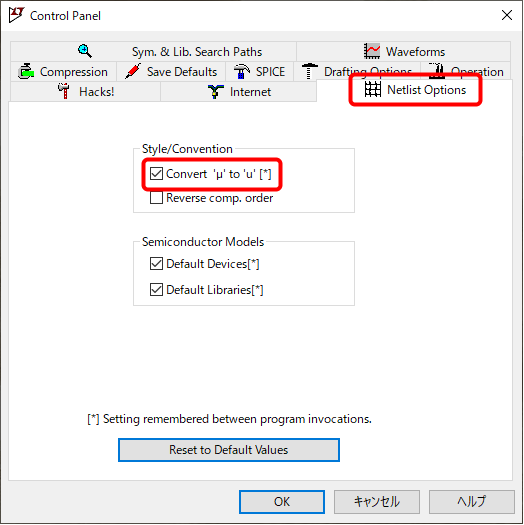
\includegraphics[width=.4\columnwidth]{img/3.png}
    }
    \caption{コントロールパネルの設定} 
    \end{center}
  \end{figure}
  \newpage
  \item 部品の追加(2SC1815)\\
  2SC1815はデフォルトではSpiceモデルが設定されていないため、Spiceモデルを追加する。
    本来は、トランジスタの仕様を確認しながらトランジスタの特性を表すための乗数をSpiceモデルで設定するが、ここでは登録の方法だけ紹介する。
    \begin{itemize}
      \item \verb|C:\Users\(ユーザ名)\ドキュメント\LTSpiceXVII\lib\cmp\standard.bjt| を
      \\開く(クリックするとLTSpiceの画面が立ち上がる。)
      \item LTspiceのエディタの一番下の行に以下を入力する。
      \begin{figure}[htb]
        \begin{center}
        \subfigure[bjtファイルの場所]{
        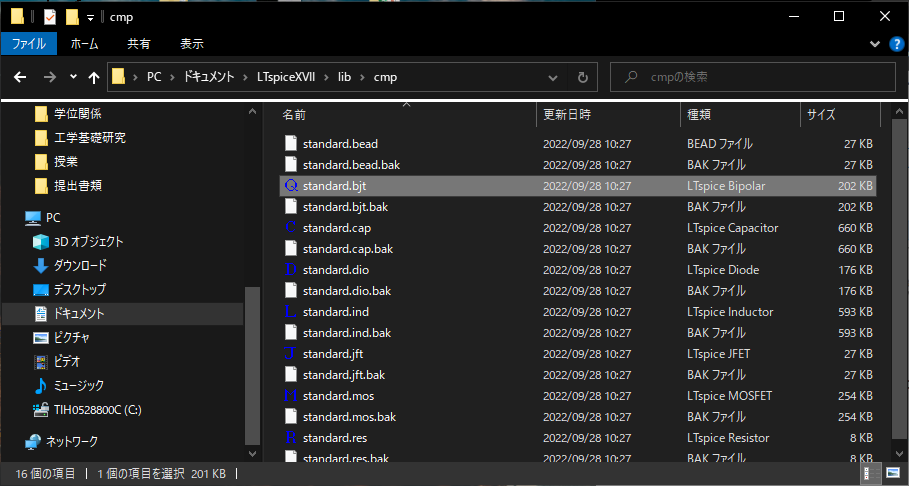
\includegraphics[width=.45\columnwidth]{img/4.png}
        }
        \subfigure[standard.bjtファイル]{
        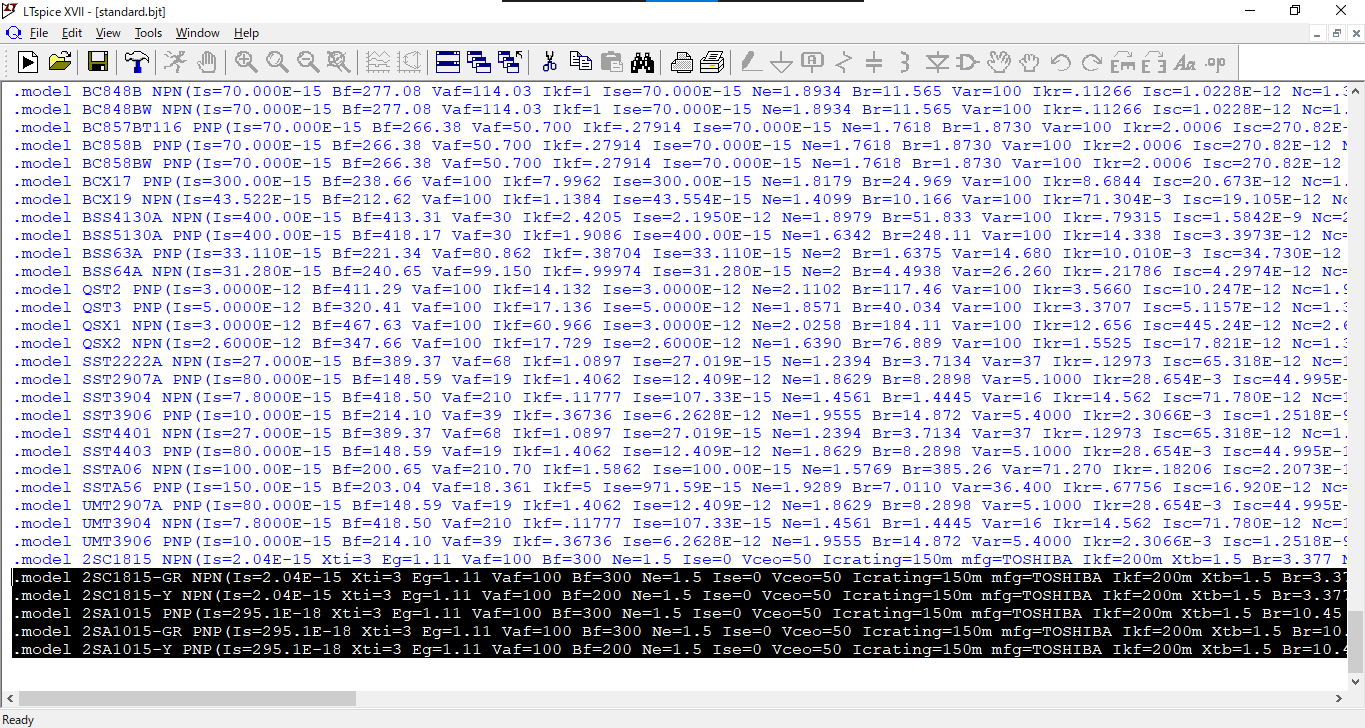
\includegraphics[width=.45\columnwidth]{img/5.png}
        }
        \caption{部品追加の設定}
        \end{center}
      \end{figure}
    \end{itemize}
\verb|.model 2SC1815-GR NPN(Is=2.04E-15 Xti=3 Eg=1.11 Vaf=100 Bf=300|\\
\verb| Ne=1.5 Ise=0 Vceo=50 Icrating=150m mfg=TOSHIBA Ikf=200m Xtb=1.5|\\
\verb| Br=3.377 Nc=2 Isc=0 Ikr=0 Rc=1 Cjc=1p Mjc=.3333| \\
\verb| Vjc=.75 Fc=.5 Cje=25p Mje=.3333 Vje=.75 Tr=450n Tf=20n Itf=0 Vtf=0 Xtf=0)|\\
\verb|.model 2SC1815-Y NPN(Is=2.04E-15 Xti=3 Eg=1.11 Vaf=100 Bf=200|\\
\verb| Ne=1.5 Ise=0 Vceo=50 Icrating=150m mfg=TOSHIBA Ikf=200m Xtb=1.5|\\
\verb| Br=3.377 Nc=2 Isc=0 Ikr=0 Rc=1 Cjc=1p Mjc=.3333|\\
\verb| Vjc=.75 Fc=.5 Cje=25p Mje=.3333 Vje=.75 Tr=450n Tf=20n Itf=0 Vtf=0 Xtf=0)|\\
\verb|.model 2SA1015 PNP(Is=295.1E-18 Xti=3 Eg=1.11 Vaf=100 Bf=300|\\ 
\verb| Ne=1.5 Ise=0 Vceo=50 Icrating=150m mfg=TOSHIBA Ikf=200m Xtb=1.5|\\
\verb| Br=10.45 Nc=2 Isc=0 Ikr=0 Rc=15 Cjc=66.2p Mjc=1.054|\\
\verb| Vjc=.75 Fc=.5 Cje=5p Mje=.3333 Vje=.75 Tr=10n Tf=1.661n Itf=0 Vtf=0 Xtf=0)|\\
\verb|.model 2SA1015-GR PNP(Is=295.1E-18 Xti=3 Eg=1.11 Vaf=100 Bf=300|\\
\verb| Ne=1.5 Ise=0 Vceo=50 Icrating=150m mfg=TOSHIBA Ikf=200m Xtb=1.5|\\
\verb| Br=10.45 Nc=2 Isc=0 Ikr=0 Rc=15 Cjc=66.2p Mjc=1.054|\\
\verb| Vjc=.75 Fc=.5 Cje=5p Mje=.3333 Vje=.75 Tr=10n Tf=1.661n Itf=0 Vtf=0 Xtf=0)|\\
\verb|.model 2SA1015-Y PNP(Is=295.1E-18 Xti=3 Eg=1.11 Vaf=100 Bf=200|\\
\verb| Ne=1.5 Ise=0 Vceo=50 Icrating=150m mfg=TOSHIBA Ikf=200m Xtb=1.5|\\
\verb| Br=10.45 Nc=2 Isc=0 Ikr=0 Rc=15 Cjc=66.2p Mjc=1.054|\\
\verb| Vjc=.75 Fc=.5 Cje=5p Mje=.3333 Vje=.75 Tr=10n Tf=1.661n Itf=0 Vtf=0 Xtf=0)|
    \begin{itemize}
      \item ファイルを保存して閉じる。
    \end{itemize}
\end{enumerate}

\subsection{基本操作}
\begin{description}
  \setlength{\parskip}{0cm} % 段落間
  \setlength{\itemsep}{0cm} % 項目間
  \item[ゴール] LTspiceの基本的な使い方を学ぶ。
  \item[キーワード] DCスイープ、DC動作点解析、過渡解析(Transient解析)、AC解析
  \item[ストーリー] ダイオードを直流電源に接続し電流を流す回路を作成する。\\ → 回路に流れる電流を解析する。(DCスイープ、DC動作点解析、過渡解析)
\end{description}

\begin{enumerate}
  \setlength{\parskip}{0cm} % 段落間
  \setlength{\itemsep}{0cm} % 項目間
  \item 新規作成、ツールバー
  \begin{figure}[htb]
    \begin{center}
    \subfigure[ツールバー]{
    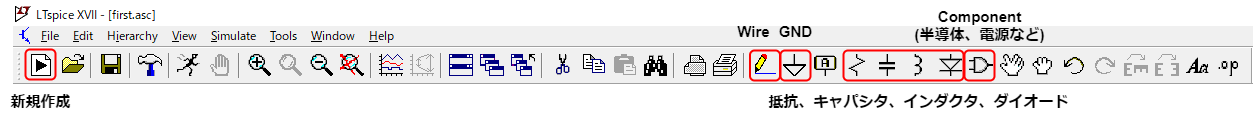
\includegraphics[width=150mm]{img/6.png}
    }
    \subfigure[電圧源の例]{
    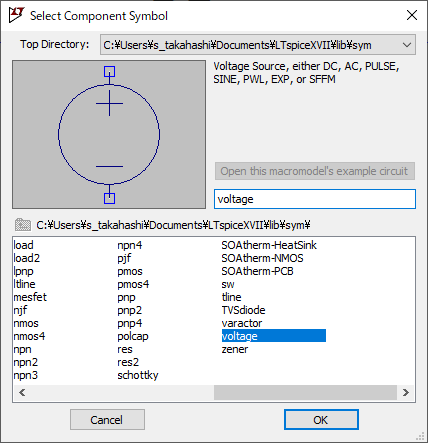
\includegraphics[width=.3\columnwidth]{img/7.png}
    }~
    \subfigure[ダイオードの選択画面]{
      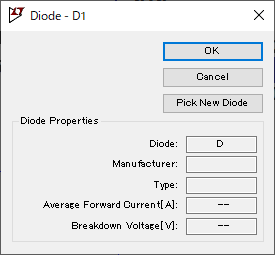
\includegraphics[width=.3\columnwidth]{img/8.png}
    }
    \caption{ツールバー詳細}
    \end{center}
  \end{figure}

  \item 部品の配置(抵抗、GND、電源) その他使い方
  \begin{itemize}
    \setlength{\parskip}{0cm} % 段落間
    \setlength{\itemsep}{0cm} % 項目間
    \item 抵抗、キャパシタ、インダクタ、ダイオードは記号をクリックすると入力できる。(または、エディタ選択中キーボードで、"R"、"L"、"C"、"D" と入力)
    \item 回路図シートで適当な位置をクリックして配置できる。
    \item Wireをクリック → 素子(シンボル)端の□をクリックして配線を接続する。
    \item 続けて同じ部品を配置しない場合は、[ESC] キー、もしくは右クリックで解除
    \item 素子値と品番は素子値を右クリックし、「Enter new Value Form」が表示されるので、入力欄に値(ダイオードの場合は品番)を入力してOKをクリックする。
    \item 向き変更、ラベルネット
    \begin{figure}[htb]
      \begin{center}
      \subfigure[向き変更]{
      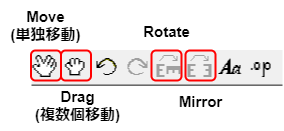
\includegraphics[width=.45\columnwidth]{img/9.png}
      }
      \subfigure[ラベルネット]{
      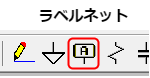
\includegraphics[width=.45\columnwidth]{img/10.png}
      }
      \caption{ツールバー詳細}
      \end{center}
    \end{figure}
    \item 保存「File」→ 「Save As」等
  \end{itemize}
\end{enumerate}
\mysubsubsection{DCスイープ(直流電流特性解析)}
回路図シート上で右クリックして、「Edit Simulation cmd」を選択、図\ref{dc}のように入力する。
Name of 1st source to sweap, Increment を入力すると、自動でSyntaxが入力される。
    \begin{figure}[htb]
      \begin{center}
      \subfigure[Edit Simulation Command]{
      
\includegraphics[height=52mm,width=.2\columnwidth]{img/11.png}
      }
      \subfigure[DCスイープディレクティブ設定]{
      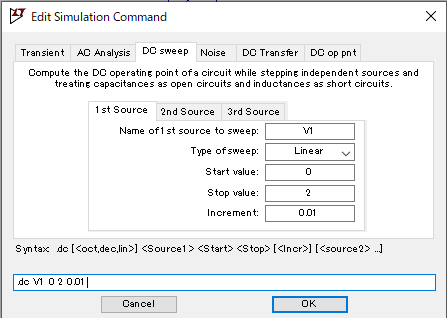
\includegraphics[width=.4\columnwidth]{img/12.png}
      }
      \caption{DCスイープ設定画面}
      \label{dc}
      \end{center}
    \end{figure}
    OKを入力すると、ディレクティブが生成されるため、回路図シートをクリックして貼り付ける。
    ディレクティブの移動は、素子等と同じ。
    「Run」ボタンをクリックすると、グラフが表示される。
    回路図シートを選択し、回路図上の任意の点にマウスカーソルを持っていくと、カーソルがプローブのアイコンに切り替わる。
    電圧、電流、電力のプローブがあり、カーソルの位置を変えるか、[ALT]キーで切り替えることができる。
    \begin{figure}[htb]
      \begin{center}
      \subfigure[DCスイープ画面]{
      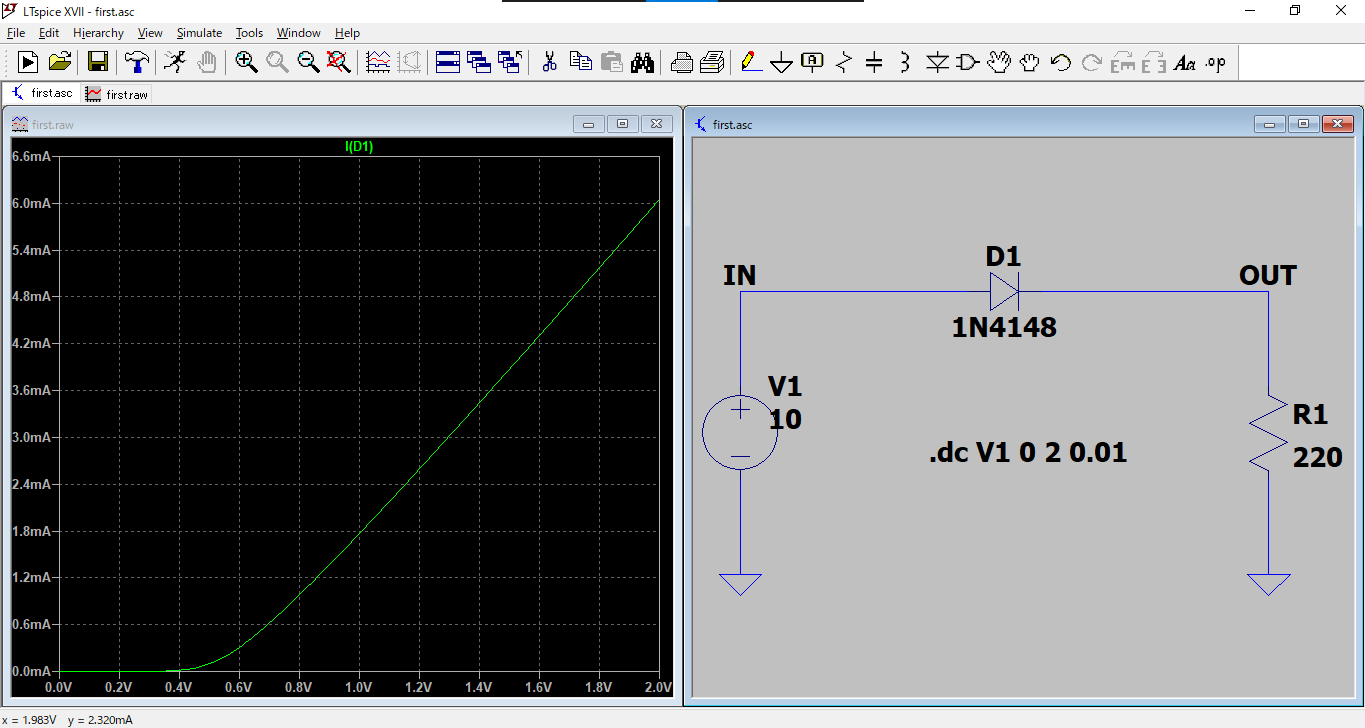
\includegraphics[width=.4\columnwidth]{img/13.png}
      }
      \subfigure[ダイオードのDC特性]{
      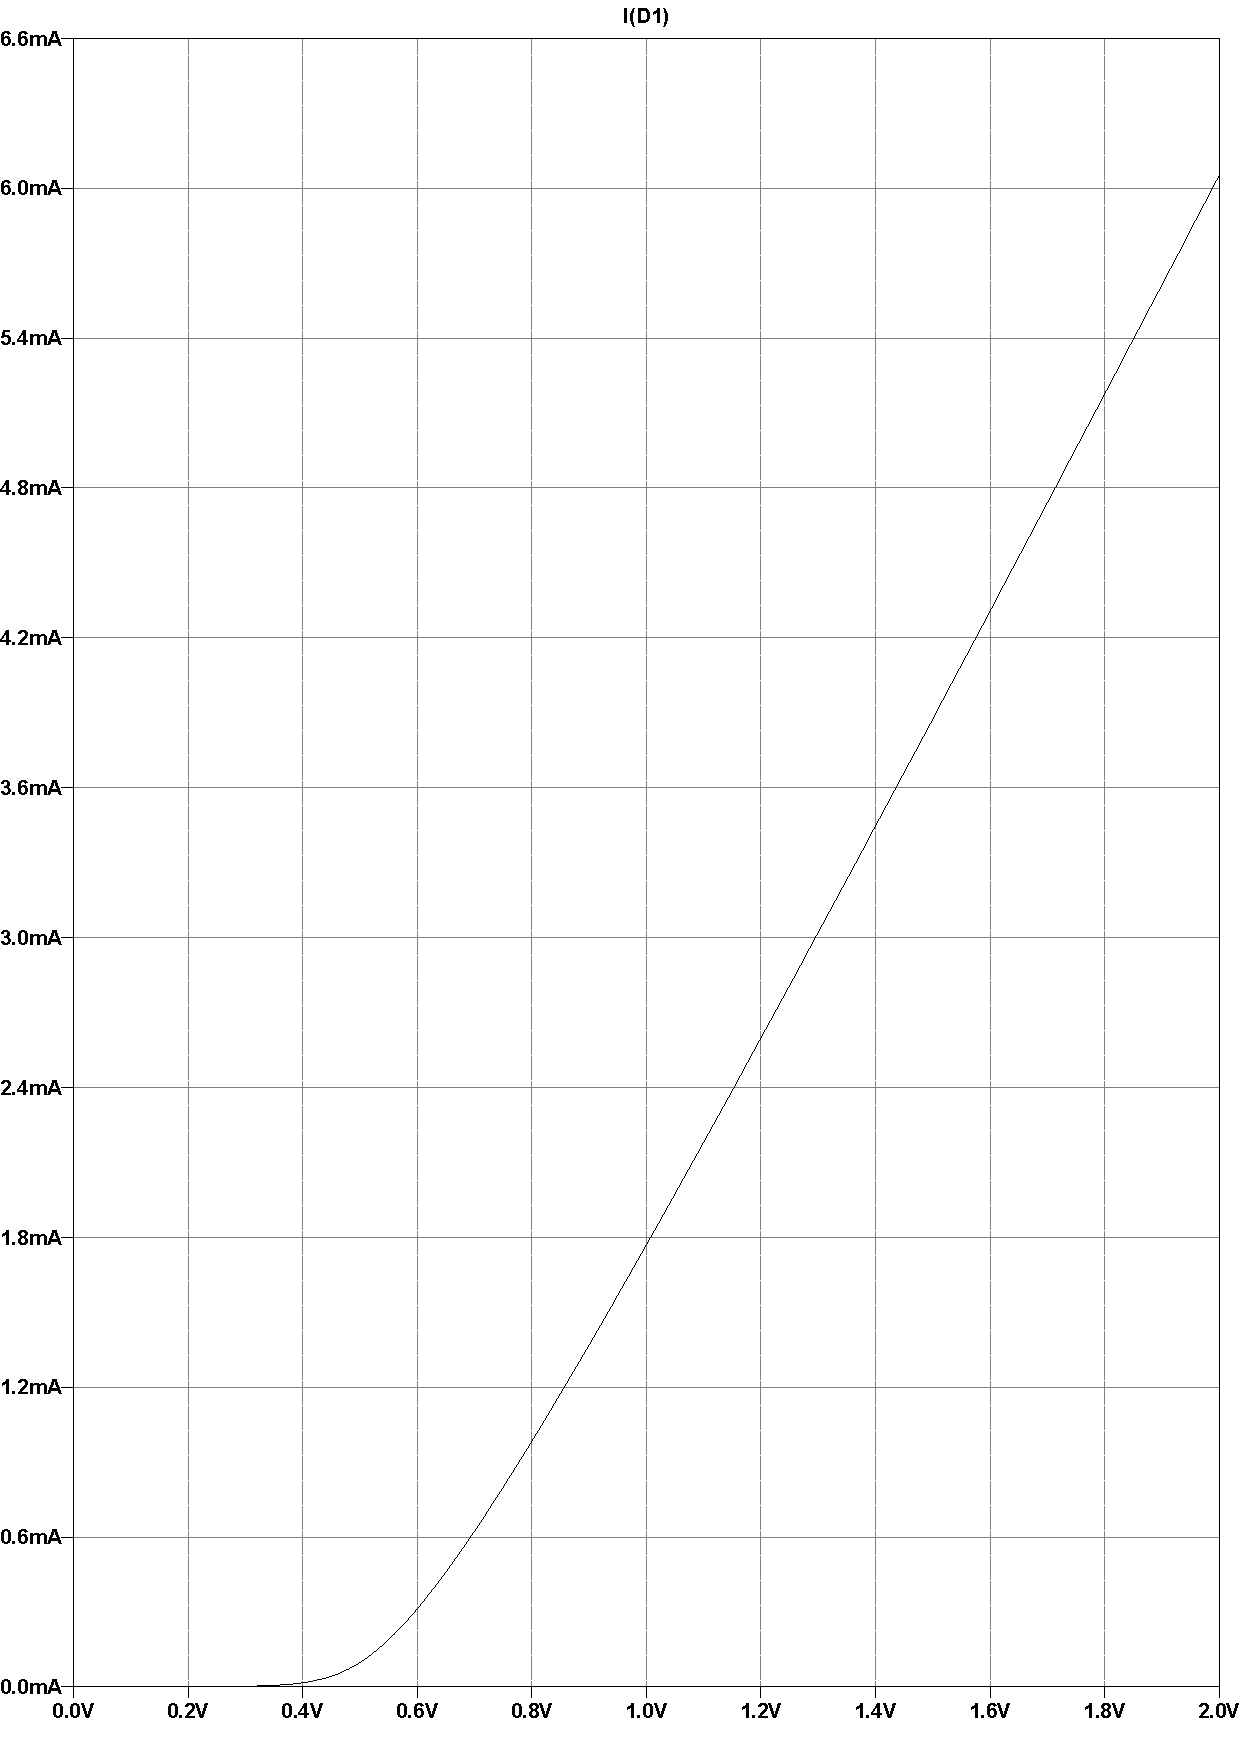
\includegraphics[width=.23\columnwidth]{img/14.pdf}
      }
      \caption{DCスイープ解析}
      \label{dckekka}
      \end{center}
    \end{figure}
\mysubsubsection{DC動作点解析}
    図\ref{dousaten}にDC動作点解析を示す。「Edit Simulation cmd」→ 「Edit Simulation Command」→ 「DC op pnt」→ OK 「.op」ディレクティブを回路図に貼り付け → 「Run」
回路各部のDC動作点(直流電圧、電流)が表示される。配線の所望箇所で右クリックして「Place .op Data Label」を選択 → 該当の電圧が表示される。
    さらに右クリックで、電圧電流の表示オプションが選択できるようになる。
    変更前の項目は\verb|「$」|で表示。これを削除して新しい項目を選択する。
    \begin{figure}[htb]
      \begin{center}
      \subfigure[Place .op Data Label]{
      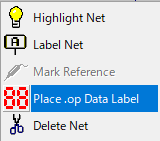
\includegraphics[width=.2\columnwidth]{img/17.png}
      }
      \subfigure[DC動作点解析結果]{
      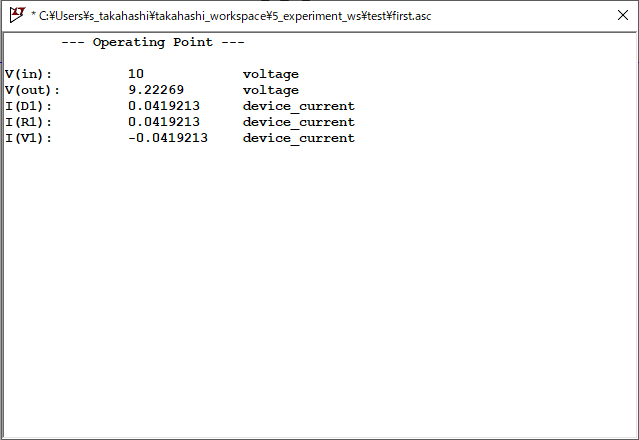
\includegraphics[width=.45\columnwidth]{img/16.png}
      }~
      \subfigure[動作点のラベル]{
        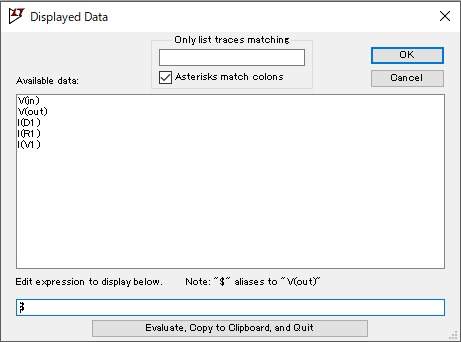
\includegraphics[width=.45\columnwidth]{img/18.png}
      }
      \caption{DC動作点解析}
      \label{dousaten}
      \end{center}
    \end{figure}
    \newpage
\subsubsection{過渡(Transient)解析}
    図\ref{kato}に、$v_1$を右クリック →「Advanced」→ "SINE" をチェックして、図のように設定する。
    「Edit Simulation cmd」→ 「Edit Simulation Command」→ 「Transient」タブ → Stop timeに "3m" を入力 → OKをクリックし、.tran ディレクティブを貼り付け → 「Run」
先に貼り付けたディレクティブはセミコロンがついて、無効化されている。
    \begin{figure}[htb]
      \begin{center}
      \subfigure[過渡解析結果]{
      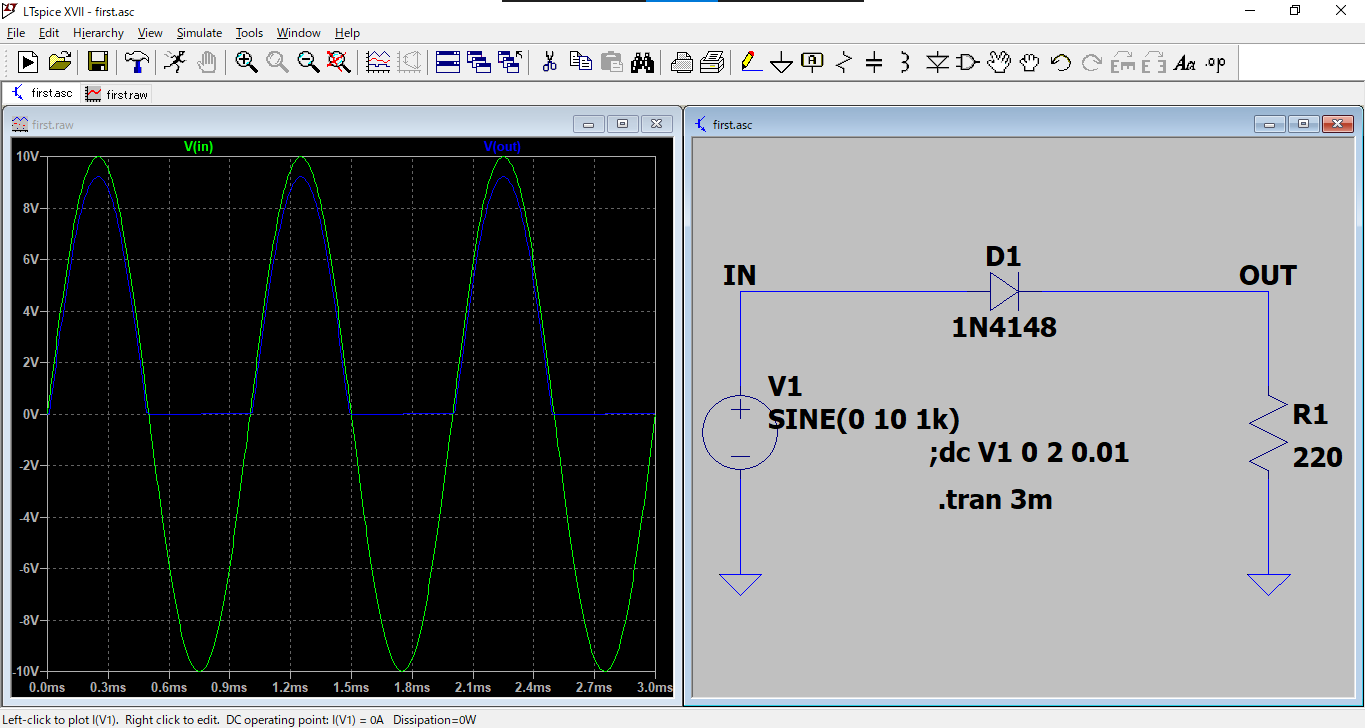
\includegraphics[width=.5\columnwidth]{img/19.png}
      }
      \subfigure[入力信号$v_1$の設定]{
      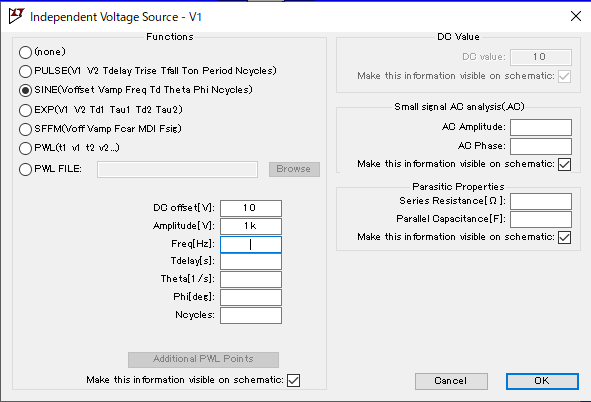
\includegraphics[width=.45\columnwidth]{img/20.png}
      }
      \caption{過渡(Transient)解析}
      \label{kato}
      \end{center}
    \end{figure}
\subsubsection{AC解析}
    図\ref{ac}にAC解析を示す。ここではRLC並列共振回路を作成しAC解析により周波数特性を取得する。
    電圧源をAC 1Vに設定する。「Edit Simultion cmd」→ 「Edit Simulation Command」→ 「AC Analysis」タブをクリック → パラメータを入力 → OK → 「.ac」ディレクティブを回路図に貼り付ける「Run」ボタンをクリックして解析を実行する。
    回路出力のOUTラベルをクリックすると、周波数特性のグラフが表示される。
    縦軸目盛がdB表示の場合、軸で「linear」を選択すると縦軸が電圧の目盛になる。
    \begin{figure}[htb]
      \begin{center}
      \subfigure[電圧源の設定]{
      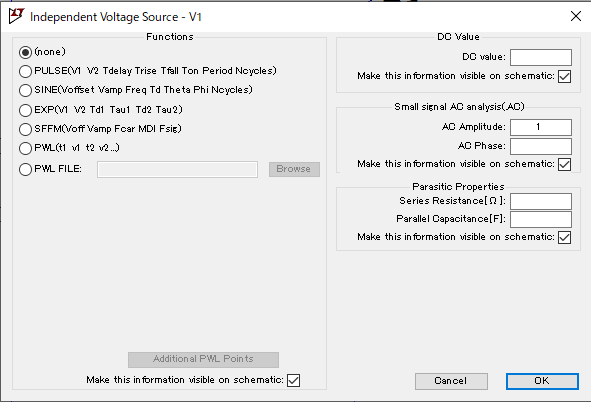
\includegraphics[width=.3\columnwidth]{img/21.png}
      }~
      \subfigure[ACディレクティブの設定]{
      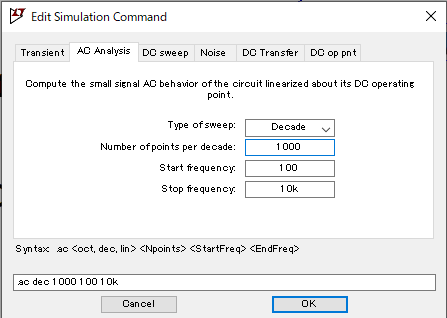
\includegraphics[width=.3\columnwidth]{img/22.png}
      }
      \subfigure[AC解析結果]{
      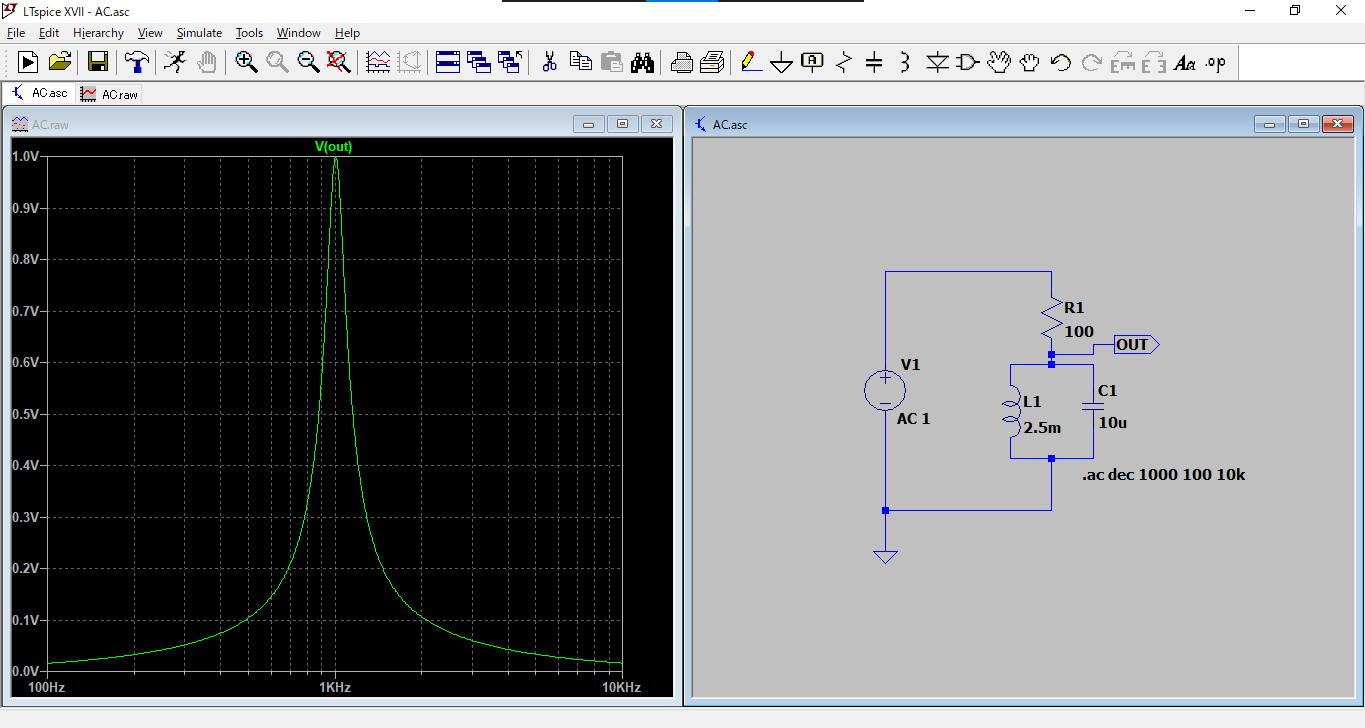
\includegraphics[width=.3\columnwidth]{img/23.png}
      }
      \caption{AC解析}
      \label{ac}
      \end{center}
    \end{figure}
    解析パラメータについて、Decadeは10倍ごとの対数目盛、Number of points は、Decade毎の計算点数、Start-Stop間の周波数を掃引(100 - 10 kHz)する。

\begin{description}
  \setlength{\parskip}{0cm} % 段落間
  \setlength{\itemsep}{0cm} % 項目間
  \item[任意課題1] これまでの操作を参考に、図\ref{diode}の回路(ダイオード回路)を作成してください。
  \item[任意課題2] 回路に流れる電流を解析して下さい。(DCスイープ、DC動作点解析、過渡解析)
  \item[任意課題3] RLC並列共振回路のAC解析を行い、(図\ref{shuhasu})共振点周波数を求めて下さい。共振点を求める式から、AC解析で入力信号を1 Vにするメリットを考えて下さい。 
  \begin{figure}[htbp]
    \begin{center}
    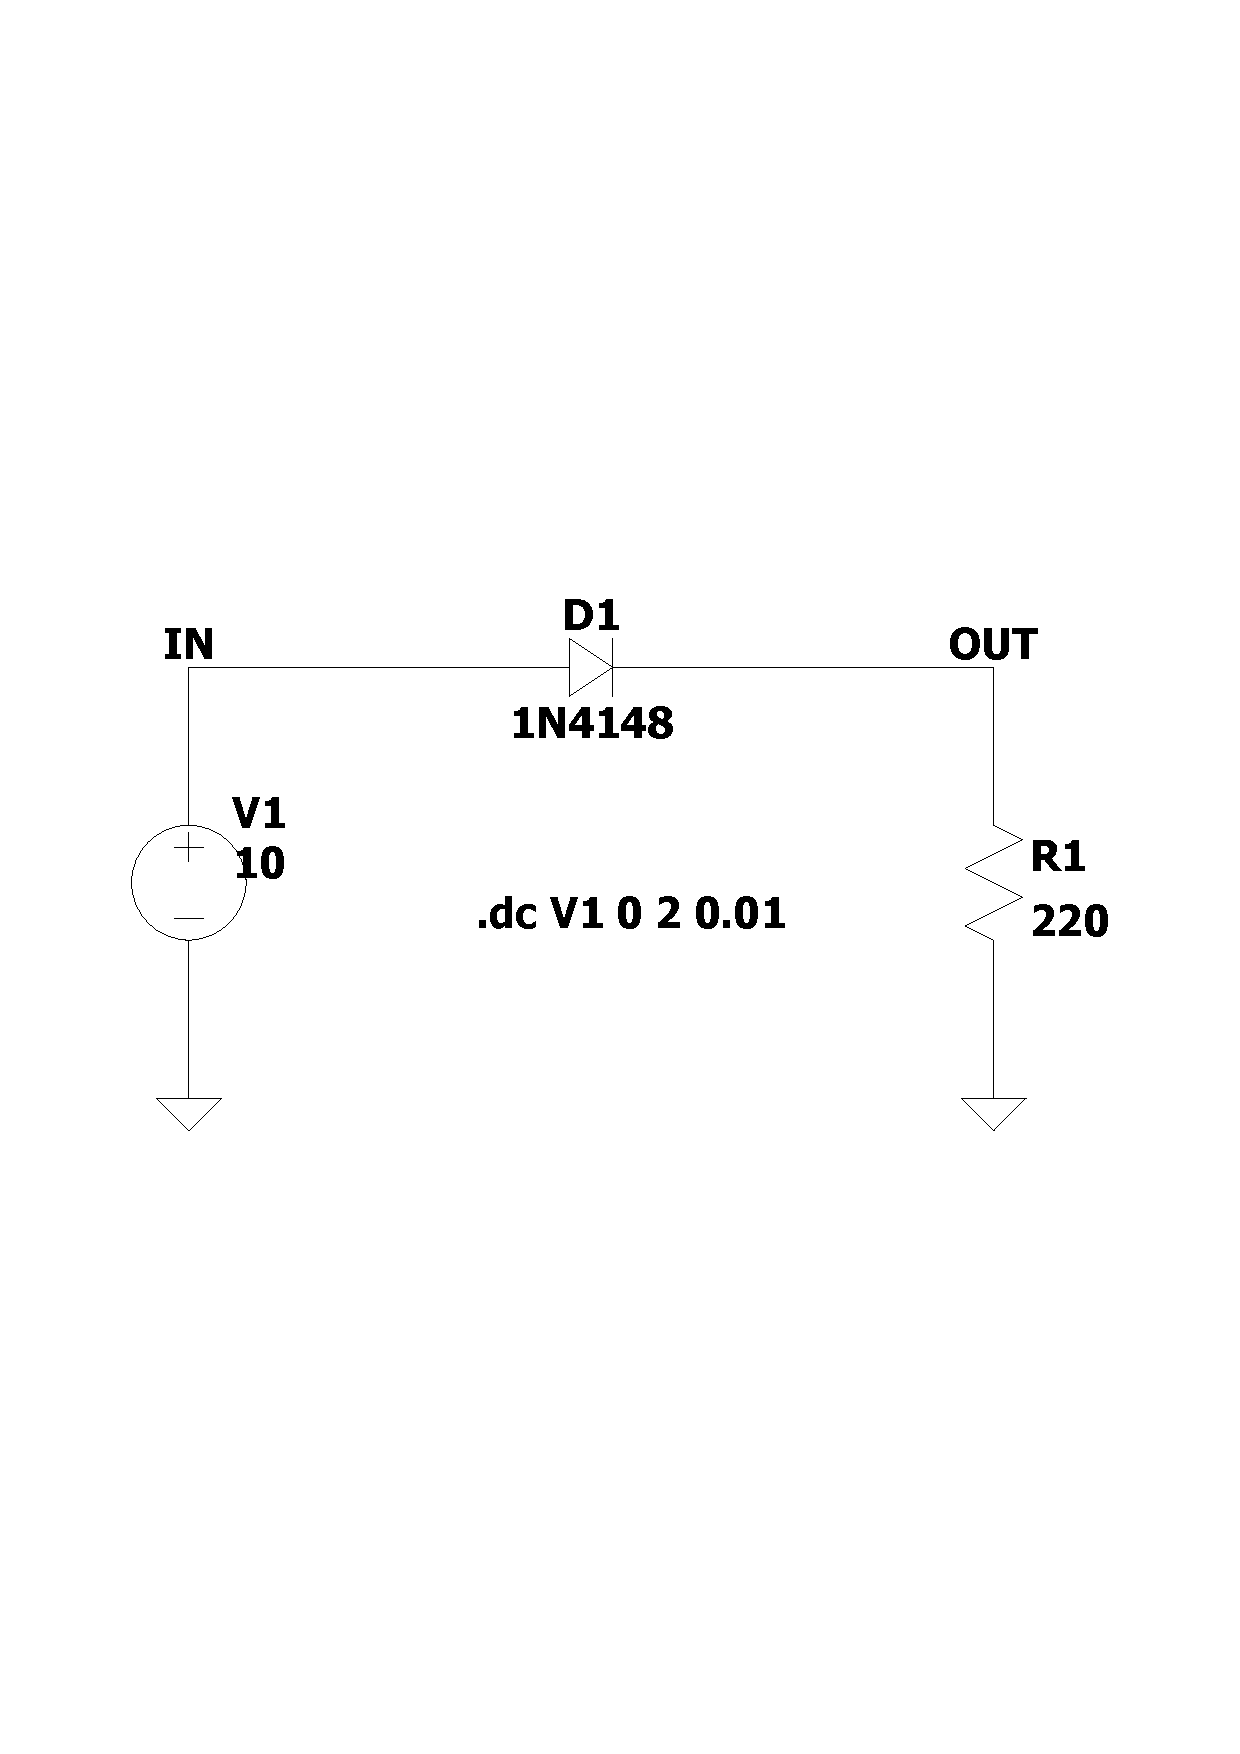
\includegraphics[width=\linewidth]{img/15.pdf}
    \caption{ダイオード回路}
    \label{diode}
    \end{center}
  \end{figure}
  \begin{figure}[htbp]
    \begin{center}
    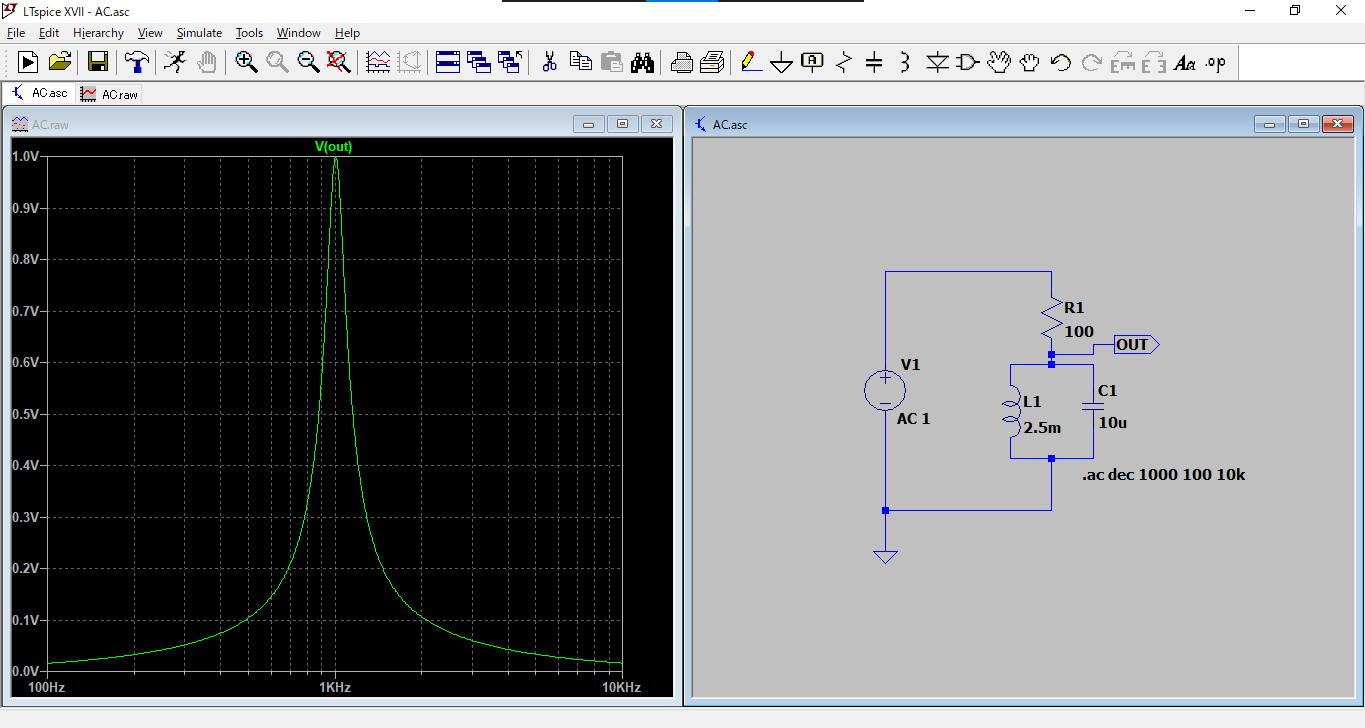
\includegraphics[width=\linewidth]{img/10_1.png}
    \caption{RLC並列共振回路のAC解析}
    \label{shuhasu}
    \end{center}
  \end{figure}
\end{description}

\end{document}